\section{Combinatorial Elastica}

\begin{frame}
\center
\huge
A combinatorial model for elastica

\vspace{2em}

\begin{minipage}{0.7\textwidth}
\normalsize
\begin{itemize}
\item{Validate that multigrid convergent estimators can be used in optimization models.}
\item{LocalSearch algorithm.}
\item{Global optimum for the free elastica.}
\end{itemize}
\end{minipage}


\end{frame}

\begin{frame}
	{Combinatorial Elastica}	
	{Digital elastica}

Continuous elastica:\hspace{1em} $\displaystyle \int_{\partial S}{ \alpha + \beta \kappa ^2ds}.$

%	
		\begin{definition}[Digital elastica energy]
		Let $\hat{\kappa}$ and $\hat{s}$ multigrid convergent estimators of curvature and local length. The digital elastica energy of a digital shape $D \subset \Omega \subset \mathbb{Z}^2$ of parameters $\vec{\theta} = (\alpha \geq 0, \beta \geq 0)$ is defined as
%		
		\begin{align*}
			\hat{E}_{\vec{\theta}}(D) = \sum_{\dot{e} \in \partial_h(D)}{\hat{s}(\dot{e}) \Big(\: \alpha + \beta \hat{\kappa}^2(\dot{e}) \: \Big). }
		\end{align*}
	\end{definition}
%	
	\begin{itemize}
		\item<2->{The digital elastica energy converges (multigrid) to the continuous elastica.}\\[2em]
		\item<3->{\emph{Local search}: set a local neighborhood $\mathcal{W}(D)$ of $D$ and pick the shape $X^{\star} \in \mathcal{W}(D)$ among those of minimum digital elastica value.}
	\end{itemize}
\end{frame}
%
%
%
%\begin{frame}
%	{Combinatorial Elastica}	
%	{Local search algorithm}
%
%\begin{algorithm}[H]
% \SetKwData{It}{i}
% \SetKwData{MIt}{maxIt}
% \SetKwData{Tol}{tolerance}
% \SetKwData{Delta}{delta}
% \SetKwData{Best}{best} 
% \SetKwInOut{Input}{input}\SetKwInOut{Output}{output}
% 
% \Input{A digital set $D$; coefficients  $\vec{\theta}=(\alpha, \beta)$; the maximum number of iterations \MIt; and a stop condition \Tol}
% \BlankLine
% \Delta $\longleftarrow$ \Tol+1\;
% $i \longleftarrow 0$\;
% $D^{(0)} \longleftarrow D$\;
% $X^\star \longleftarrow D$\;
% \While{ \color{black} \It $<$ \MIt \bf{and} \Delta $>$ \Tol  }{
%  	\For{$\color{black} X \in \mathcal{W}(S^{(i)}) $}
%	{
%		\If{\color{black} $\hat{E}_{\vec{\theta}}(D)$ $<$ $\hat{E}_{\vec{\theta}}(X^\star)$ }
%		{
%			$X^\star \longleftarrow X$
%		}
%	}
%	$D^{(i+1)} \longleftarrow X^\star$\;
%	\Delta $\longleftarrow$ $\hat{E}_{\vec{\theta}}(D^{(i)}) - \hat{E}_{\vec{\theta}}(D^{(i+1)})$\;	
%	\It $\longleftarrow$ \It $+1$\;
% }
%\end{algorithm}
%\end{frame}
%
%
%
\begin{frame}
	{Combinatorial Elastica}	
	{Neighborhood of shapes}
	
\begin{itemize}
\item{Members of $\mathcal{W}(D)$ are constructed by removing or adding a set of connected pixels to $D$.}
\end{itemize}	
	
\begin{minipage}[t][0.5\textheight]{1\textwidth}
\begin{center}
\begin{tabular}{cc}
\only<1>{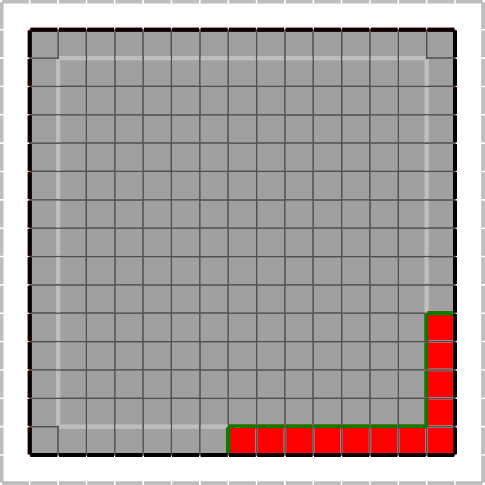
\includegraphics[scale=0.25]{figures/combinatorial-elastica/main-inner.png}}
\only<2->{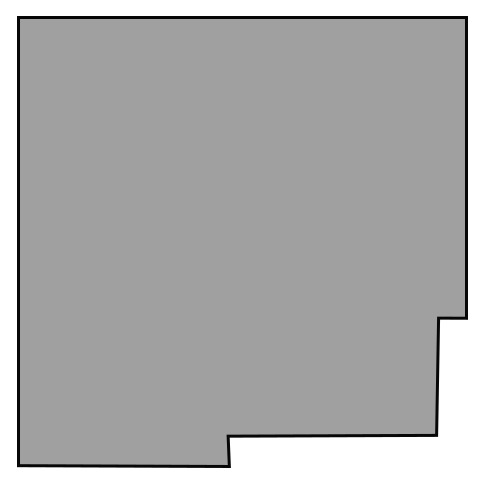
\includegraphics[scale=0.25]{figures/combinatorial-elastica/main-inner-block.png}}&
\only<1>{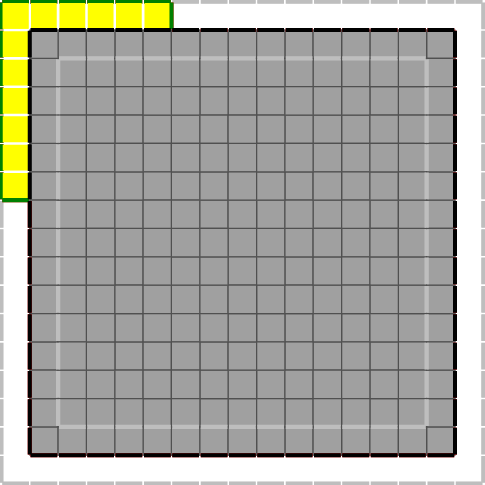
\includegraphics[scale=0.25]{figures/combinatorial-elastica/main-outer.png}}
\only<2->{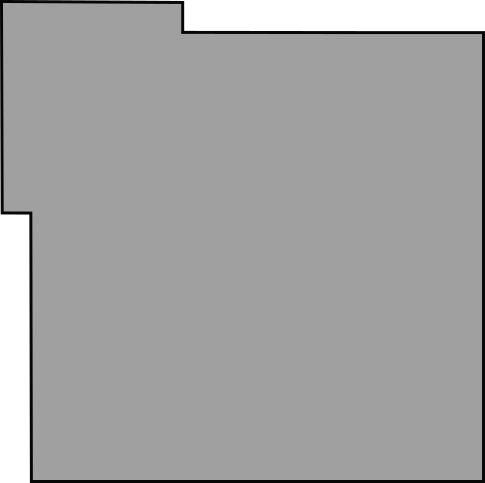
\includegraphics[scale=0.25]{figures/combinatorial-elastica/main-outer-block.png}}
\end{tabular}
\end{center}	
\end{minipage}

\onslide<3->{
\[
\begin{array}{ll}
D^{(k+1)} &\longleftarrow \displaystyle \argmin_{X \in \mathcal{W}(D^{(k)})}\hat{E}_{\vec{\theta}}(X).
\end{array}
\]
}

\onslide<3>{
\begin{itemize}
\item{We use the integral invariant estimator (II-r) to estimate the curvature.}
\end{itemize}}

\end{frame}

\begin{frame}
	{Combinatorial Elastica}	
	{Free elastica}

Free elastica: \hspace{1em}
\[
\begin{array}{ll}
D^{(k+1)} &\longleftarrow \displaystyle \argmin_{X \in \mathcal{W}(D^{(k)})}\hat{E}_{\vec{\theta}}(X).
\end{array}
\]	
	
\begin{center}
\begin{tabular}{ccc}
\multirow{4}{*}{$D^{(0)}$} & 
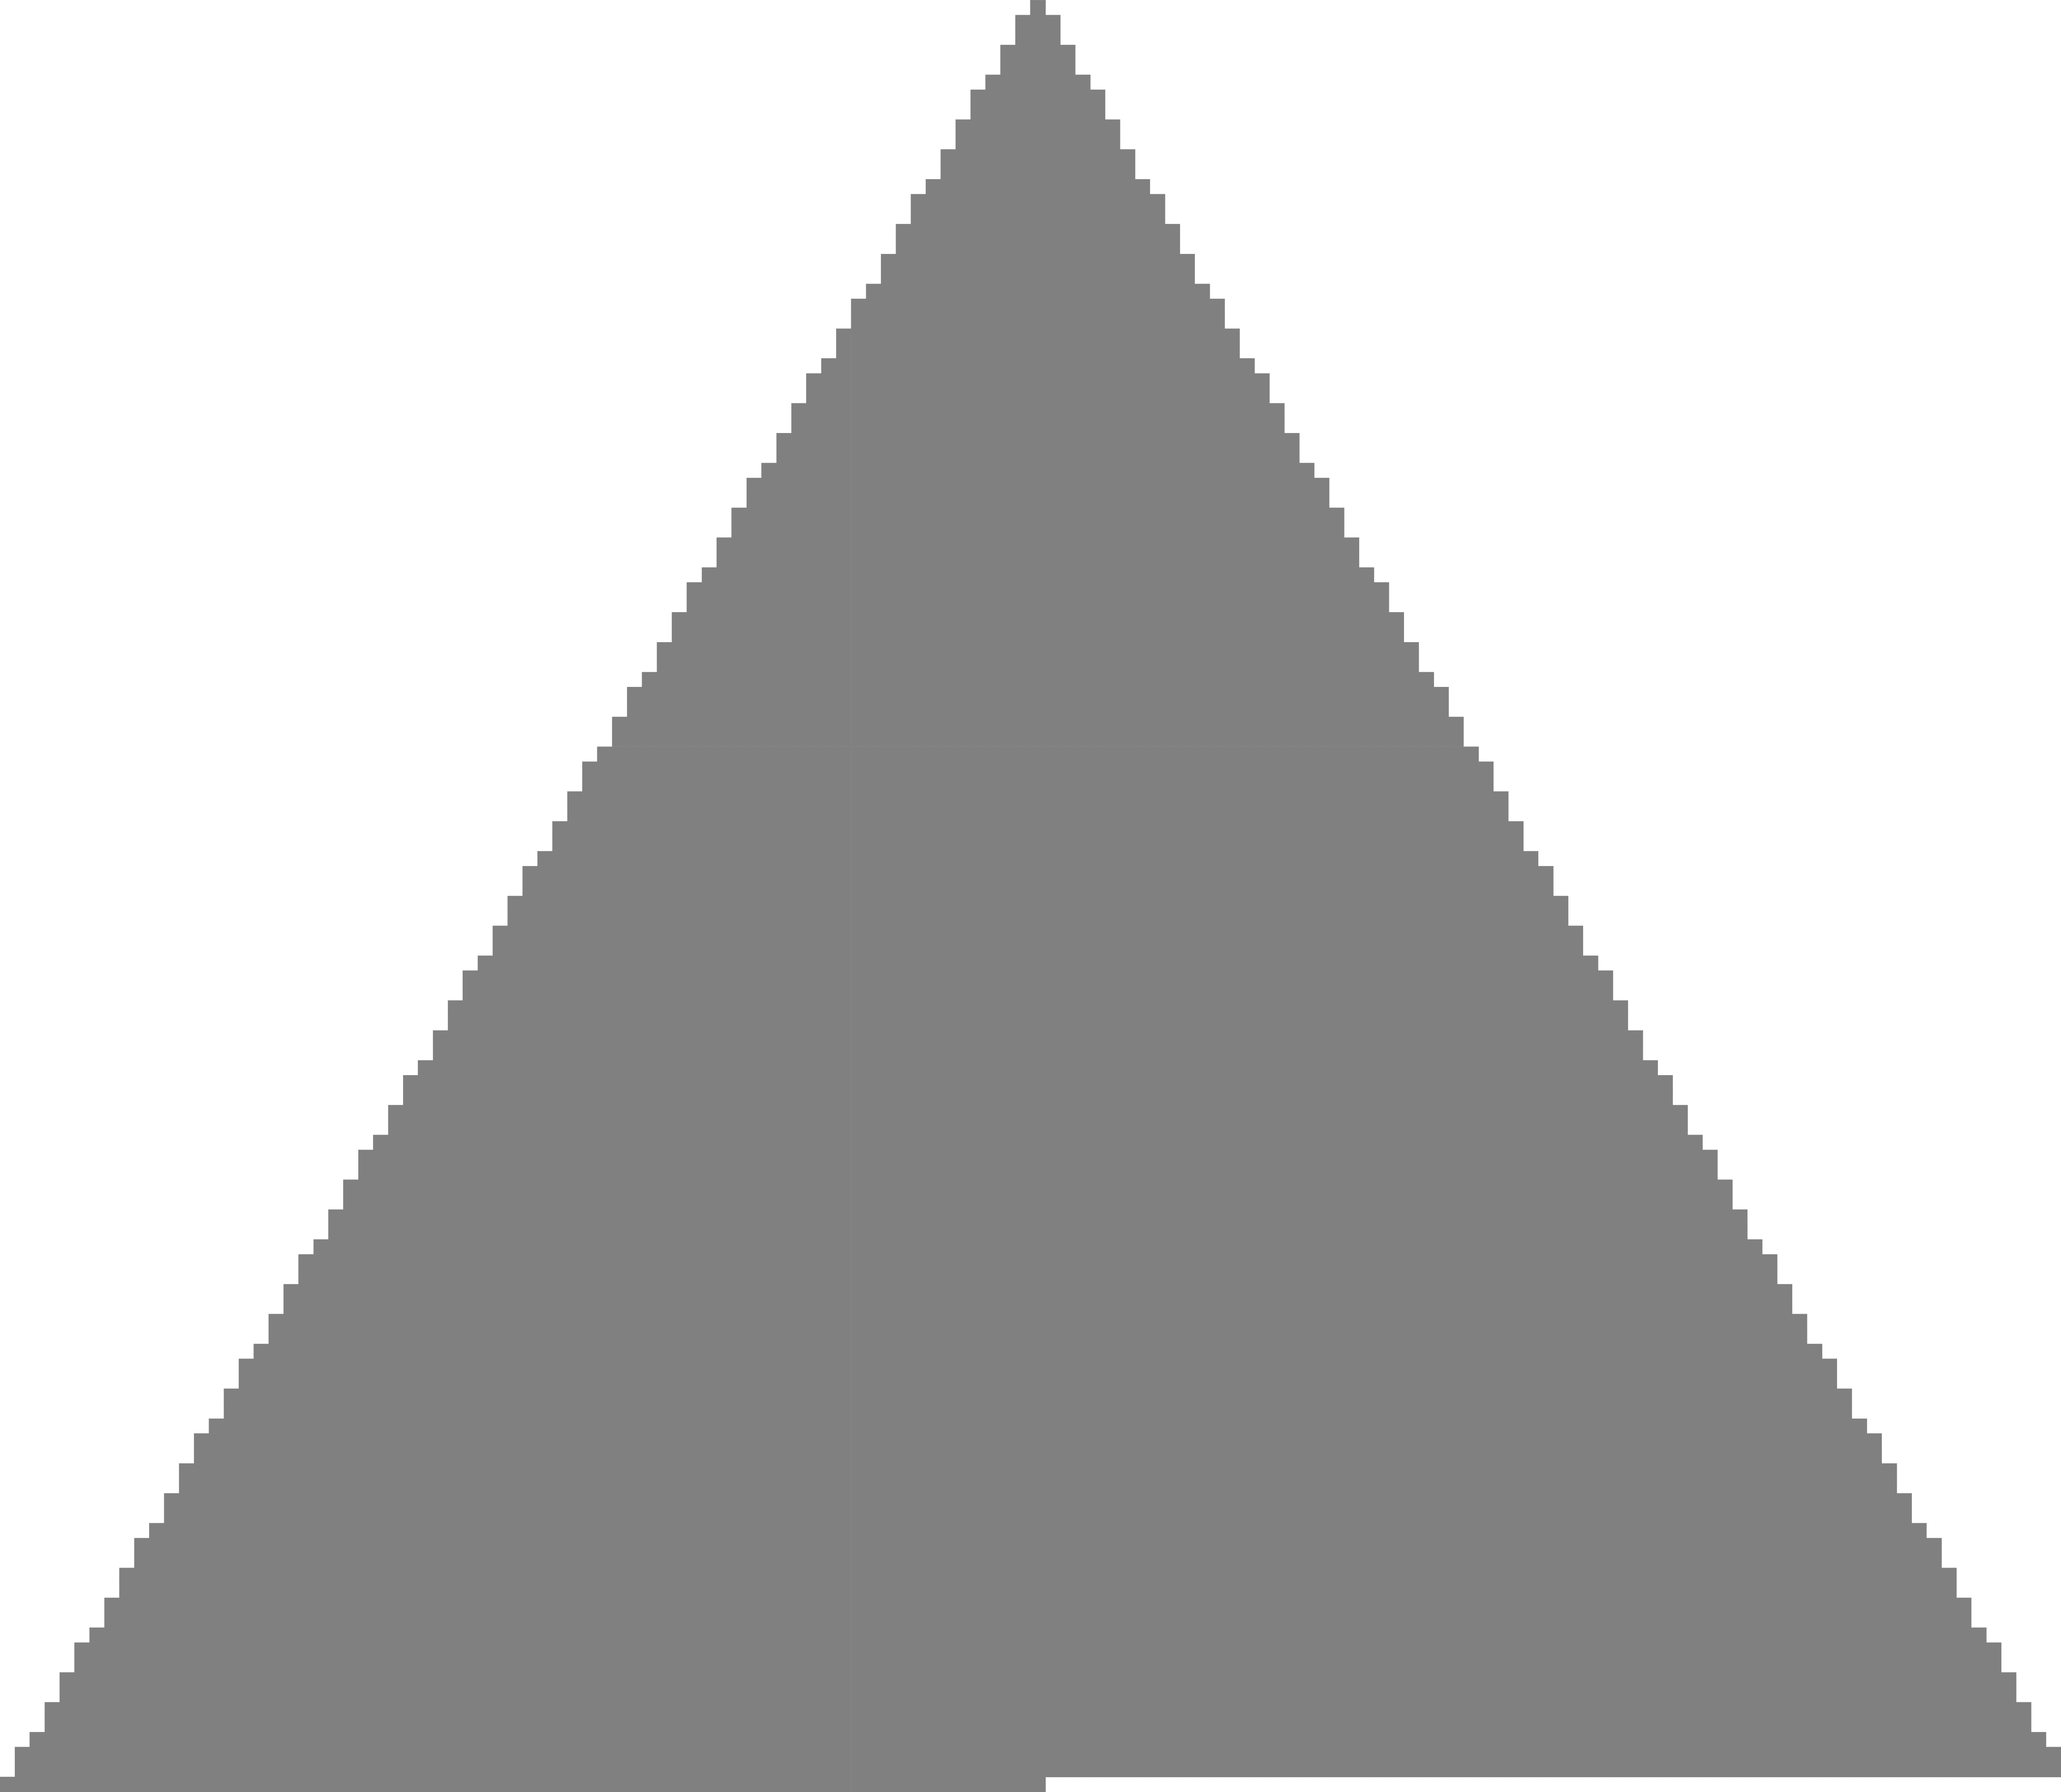
\includegraphics[scale=0.015]{figures/combinatorial-elastica/shapes/triangle.png}&

\includegraphics[scale=0.015]{figures/combinatorial-elastica/shapes/square.png}\\
&Triangle & Square\\[1.5em]
& 
\includegraphics[scale=0.01]{figures/combinatorial-elastica/shapes/flower.png}&

\includegraphics[scale=0.01]{figures/combinatorial-elastica/shapes/bean.png}\\
& Flower & Bean
\end{tabular}		
\end{center}

\end{frame}

\begin{frame}
	{Combinatorial Elastica}	
	{Free elastica evolution}

\begin{center}
{\footnotesize
\[
\hat{E}_{\vec{\theta}}(D) = \sum_{\dot{e} \in \partial_h(D)}{\hat{s}(\dot{e}) \Big(\: \alpha + \beta \hat{\kappa}^2(\dot{e}) \: \Big). }\]
}\\

II-$5$, $\alpha=0.01, \beta=1.$
\end{center}
\begin{minipage}{0.49\textwidth}
\center
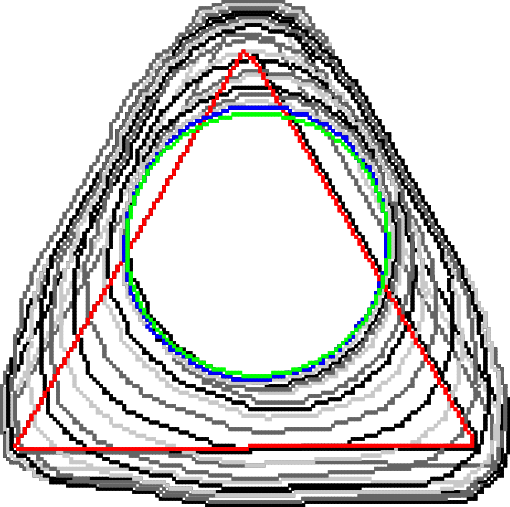
\includegraphics[scale=0.15]{figures/combinatorial-elastica/flow/ii/elastica/len_pen_0.01000/jonctions_1/curve_segs_4/best/gs_0.25000/triangle.png}\\[1em]
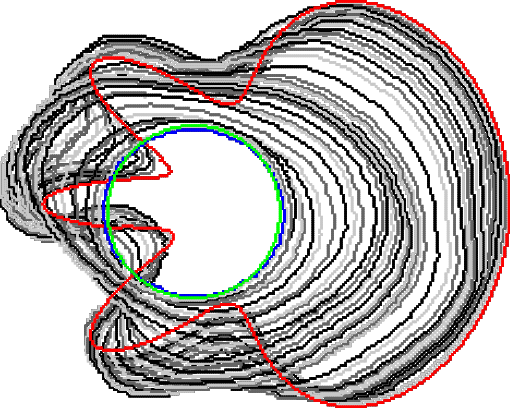
\includegraphics[scale=0.18]{figures/combinatorial-elastica/flow/ii/elastica/len_pen_0.01000/jonctions_1/curve_segs_4/best/gs_0.25000/flower.png}
\end{minipage}	
\begin{minipage}{0.49\textwidth}
\center
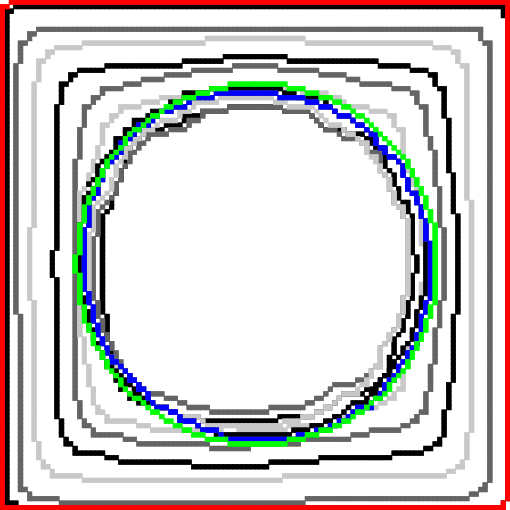
\includegraphics[scale=0.15]{figures/combinatorial-elastica/flow/ii/elastica/len_pen_0.01000/jonctions_1/curve_segs_4/best/gs_0.25000/square.png}\\[1em]
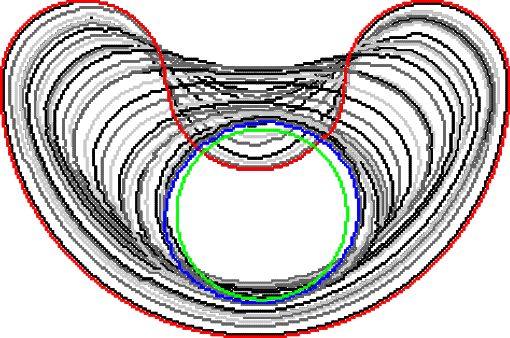
\includegraphics[scale=0.18]{figures/combinatorial-elastica/flow/ii/elastica/len_pen_0.01000/jonctions_1/curve_segs_4/best/gs_0.25000/bean.png}
\end{minipage}

\end{frame}

\begin{frame}
	{Combinatorial Elastica}	
	{Energy evolution}

\begin{minipage}{0.49\textwidth}
\center
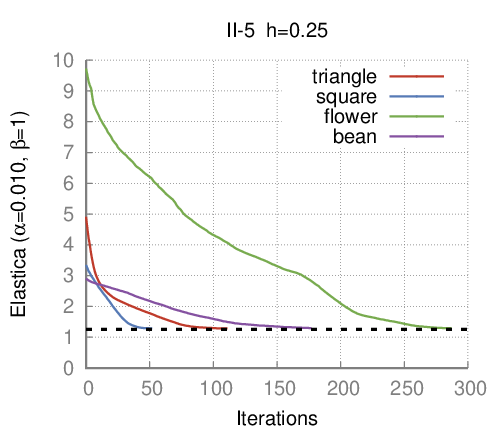
\includegraphics[scale=0.3]{figures/combinatorial-elastica/flow/ii/elastica/len_pen_0.01000/jonctions_1/curve_segs_4/best/gs_0.25000/summary-ii5.png}
\end{minipage}
\begin{minipage}{0.5\textwidth}
\small
\begin{align*}
	\min E(X) &= \int_{\partial X}{ \alpha + \beta \kappa^2 ds}\\
	 &= 4\pi \beta \frac{1}{r} = 4\pi \beta \left(\frac{\alpha}{\beta}\right)^{1/2},
\end{align*}
where $\frac{\partial }{\partial r} 2\pi(\alpha r + \frac{\beta}{r}) = 0.$\\ 

%
For $\alpha=0.01,\; \beta=1,$
%
\begin{align*}
	\min E(X) \approx 1.2566.
\end{align*}
\end{minipage}

\vspace{1em}

\onslide<2>{
\begin{itemize}
\item{What is the influence of the radius of the estimation disk?}
\end{itemize}
}
	
\end{frame}

\begin{frame}
	{Combinatorial Elastica}
	{Radius and grid resolution}
	
\begin{minipage}{0.49\textwidth}
\center
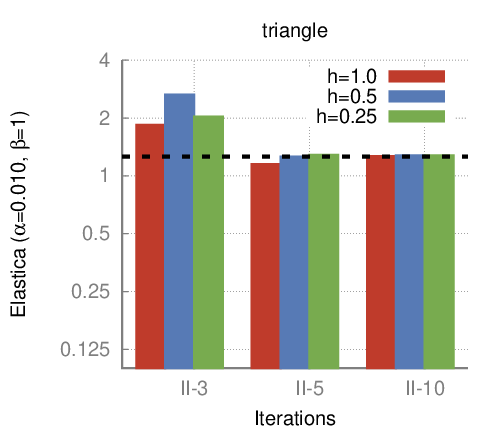
\includegraphics[scale=0.25]{figures/combinatorial-elastica/flow/ii/elastica/len_pen_0.01000/jonctions_1/curve_segs_4/best/gs_0.25000/triangle-bars.png}\\[0.6em]
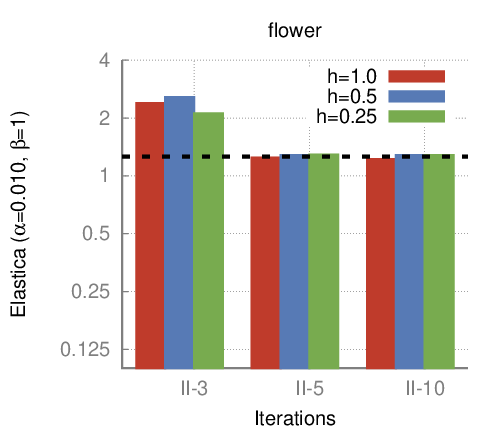
\includegraphics[scale=0.25]{figures/combinatorial-elastica/flow/ii/elastica/len_pen_0.01000/jonctions_1/curve_segs_4/best/gs_0.25000/flower-bars.png}
\end{minipage}	
\begin{minipage}{0.49\textwidth}
\center
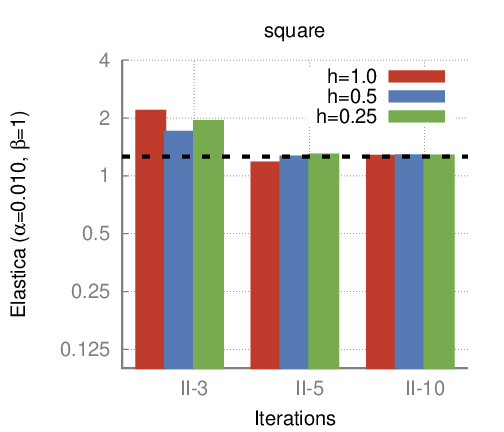
\includegraphics[scale=0.25]{figures/combinatorial-elastica/flow/ii/elastica/len_pen_0.01000/jonctions_1/curve_segs_4/best/gs_0.25000/square-bars.png}\\[0.6em]
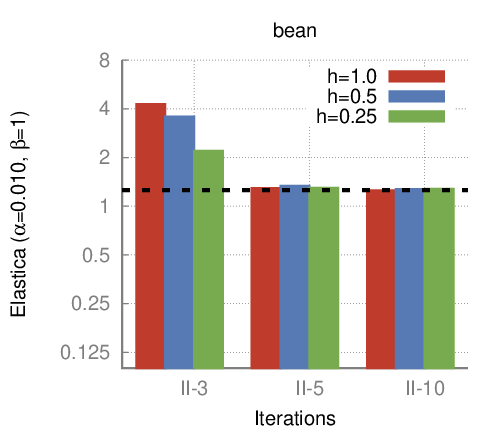
\includegraphics[scale=0.25]{figures/combinatorial-elastica/flow/ii/elastica/len_pen_0.01000/jonctions_1/curve_segs_4/best/gs_0.25000/bean-bars.png}
\end{minipage}

\onslide<2>{
\begin{figure}
\begin{tikzpicture}[overlay, remember picture] 
\node at (current page.north east) 
    [
    anchor=center,
    xshift=-35mm,
    yshift=-30mm
    ] 
{

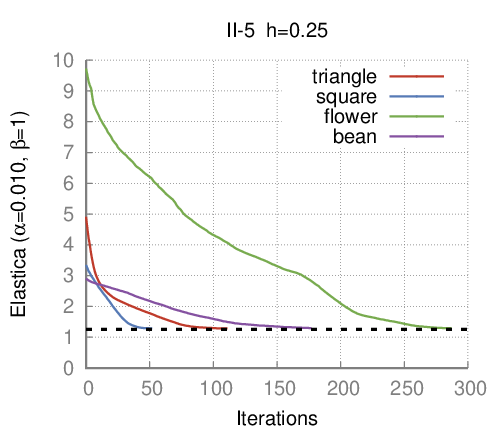
\includegraphics[scale=0.4]{figures/combinatorial-elastica/flow/ii/elastica/len_pen_0.01000/jonctions_1/curve_segs_4/best/gs_0.25000/summary-ii5.png}
	
};
\end{tikzpicture}	
\end{figure}	
}

\end{frame}

\begin{frame}
	{Combinatorial Elastica}
	{Other experiments}
\begin{center}
{\footnotesize
\[
\hat{E}_{\vec{\theta}}(D) = \sum_{\dot{e} \in \partial_h(D)}{\hat{s}(\dot{e}) \Big(\: \alpha + \beta \hat{\kappa}^2(\dot{e}) \: \Big). }\]
}\\

II-$10$, $\alpha=0.001, \beta=1.$

\vspace{1em}
	
\begin{tabular}{cc}
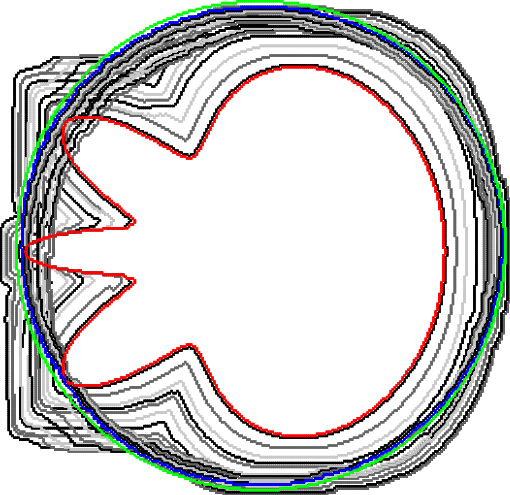
\includegraphics[scale=0.25]{figures/combinatorial-elastica/other-experiments/ii/elastica/len_pen_0.001000/jonctions_1/curve_segs_4/best/gs_0.25000/flower.png}&
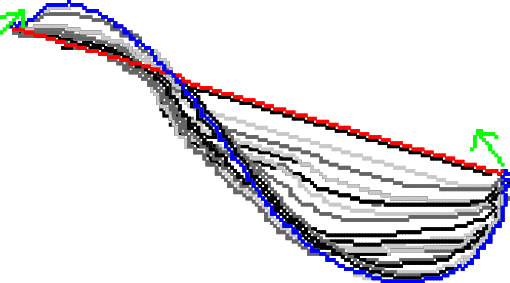
\includegraphics[scale=0.25]{figures/combinatorial-elastica/other-experiments/ii/elastica/len_pen_0.001000/jonctions_1/curve_segs_4/best/gs_0.25000/curve.png}\\
Free elastica. & Constrained elastica.
\end{tabular}
\end{center}

\vspace{1em}
\pause

\begin{itemize}
\item{What about running time?}
\end{itemize}

\end{frame}

\begin{frame}
{Combinatorial Elastica}
{Running time}
\begin{center}
\captionsetup{type=table}
\scriptsize
\begin{tabular}{|l|c|c|c|c|c|c|}
\hline
& \multicolumn{2}{c|}{$h=1.0$} & \multicolumn{2}{c|}{$h=0.5$} & \multicolumn{2}{c|}{$h=0.25$}\\
\hline
& Pixels & Time & Pixels & Time & Pixels & Time\\
\hline
Triangle & 521 & 2s (0.07s/it)  & 2080 & 43s (0.81s/it) & 8315 & 532s(4.8s/it)\\
{\color{highlightcolor}Square} & 841 & 0.9s (0.09s/it) & 3249 & 8s (0.3s/it) & {\color{highlightcolor}12769} & {\color{highlightcolor}102s (2s/it)}\\
{\color{highlightcolor}Flower} & 1641 & 13s (0.24s/it) & 6577 & 209s (1.68s/it) & {\color{highlightcolor}26321} & {\color{highlightcolor}3534s (12.3s/it)}\\
Bean  & 1574 & 7s (0.16s/it) & 6278 & 88s (1.08s/it) & 25130 & 1131s (6.4s/it)\\
Ellipse  & 626 & 1s (0.14s/it) & 2506 & 16s (0.44s/it) & 10038 & 286s (3.1s/it)\\
\hline
\end{tabular}
\caption{\textbf{Running time for the free elastica problem.} Quite high running times. The geometry of the shape influences in the total running time.}
\end{center}
\end{frame}

\begin{frame}
{Combinatorial Elastica}
{Conclusion}

\begin{itemize}
\item{Multigrid convergent estimators are suitable for elastica minimization}\\[1em]
\item{A simple neighborhood is sufficient to escape bad local minimum. Some solutions are very close to global optimum.}\\[1em]
\item{Too slow. It cannot be used in practice.}
\end{itemize}
\end{frame}